\documentclass[a4paper,11pt,twoside]{article}
%\documentclass[a4paper,11pt,twoside,se]{article}

\usepackage{UmUStudentReport}
\usepackage{verbatim}   % Multi-line comments using \begin{comment}
\usepackage{courier}    % Nicer fonts are used. (not necessary)
\usepackage{pslatex}    % Also nicer fonts. (not necessary)
\usepackage[pdftex]{graphicx}   % allows including pdf figures
\usepackage{listings}
\usepackage{pgf-umlcd}
%\usepackage{lmodern}   % Optional fonts. (not necessary)
%\usepackage{tabularx}
%\usepackage{microtype} % Provides some typographic improvements over default settings
%\usepackage{placeins}  % For aligning images with \FloatBarrier
%\usepackage{booktabs}  % For nice-looking tables
%\usepackage{titlesec}  % More granular control of sections.

% DOCUMENT INFO
% =============
\department{Department of Computing Science}
\coursename{Object-Oriented Programming Methodology 7.5 p}
\coursecode{5DV133}
\title{OU4 Sensor Network}
\author{Johan Eklund ({\tt{kv03jed@cs.umu.se}}) \\ 
Tommie Lindberg ({\tt{c15tlg@cs.umu.se}}) \\
Jakob Lundin ({\tt{c14jln@cs.umu.se}}) \\
Lorenz Gerber ({\tt{dv15lgr@cs.umu.se}}, {\tt{lozger03@student.umu.se}})
}
\date{2016-05-23}
%\revisiondate{2016-01-18}
\instructor{Anders Broberg \\ Niklas Fries \\ Adam Dahlgren \\
  Jonathan Westin \\ Erik Moström \\ Alexander Sutherland}


% DOCUMENT SETTINGS
% =================
\bibliographystyle{plain}
%\bibliographystyle{ieee}
\pagestyle{fancy}
\raggedbottom
\setcounter{secnumdepth}{2}
\setcounter{tocdepth}{2}
%\graphicspath{{images/}}   %Path for images

\usepackage{float}
\floatstyle{ruled}
\newfloat{listing}{thp}{lop}
\floatname{listing}{Listing}



% DEFINES
% =======
%\newcommand{\mycommand}{<latex code>}

% DOCUMENT
% ========
\begin{document}
\lstset{language=C}
\maketitle
\thispagestyle{empty}
\newpage
\tableofcontents
\thispagestyle{empty}
\newpage

\clearpage
\pagenumbering{arabic}

\section{Introduction} 
The assignment was described on the course homepage
\cite{sensornetwork}. The aim was to implement software that
allows to perform experiments on sensor networks as described in
Braginsky and Estrin \cite{braginsky2002}. The main topic of
\cite{braginsky2002} is the use of \textit{rumour routing} as an
energy saving message transportation algorithm that for example
be used in environment surveillance networks.

The physical setup to be modelled consists of a number of autonomous
sensor nodes with a limited  signal send/receive range. Simplified it
can be said that a networking algorithm shall defome how to spread 
information of a detected event from nodes of event origin to the rest
of the network. Two simple algorithms to either spread or demand
information is spoofing. Here for example after detecting an event,
the node sends the information further to every to him known node, and
the next node will to the same. This will result in a large amount of
redundancy hence it is not very energy saving. The same is true for
requesting information about an event in this way, by sending out an
information request to every known node.

Braginsky and Estrin \cite{braginsky2002} propose an algorithm called
rumour routing. It uses two different types of messages that are sent
around the network. The first time, `agents' are generated at the
origin node of an event. They are used to spread information about
events. This is possible by maintaining routing tables to events both
in sensor nodes and in agents. Each agent knows from the beginning
`his' own event but will likely learn and spread information about
other events while travelling the net. Second, to obtain information,
`query' messages can be generated by specified nodes. They roam the
network, trying to find a node that knows the path to the event of
interest. In our implementation, this is called the `search' mode. As
soon as the `query' messages passes a node that knows the routing,
it changes to `track' mode until arriving at the destination query
that has the information about the event of interest. Then the query
message backtracks to the node of origin to report about the event. 


\section{Compiling and Running of the Program}

The program is writtne according to Java 1.7 and compiles on the
commandline with standard command \texttt{javac RumourRoutingApp.java}.
Invoking the compiled program is done by calling \texttt{java
  ./RumourRoutingApp.class} from the command line.
A typical run will result in screen output similar to the following:
\begin{verbatim}
Event at x: 30 y 120, at time 1135, id 317 
Event at x: 210 y 20, at time 1040, id 286 
Event at x: 0 y 50, at time 1422, id 389 
Event at x: 150 y 250, at time 1410, id 385 
Event at x: 130 y 0, at time 1826, id 490 
Event at x: 130 y 220, at time 3002, id 748 
Event at x: 50 y 270, at time 4546, id 1164 
Event at x: 130 y 210, at time 3848, id 977 
Experiment finished
\end{verbatim}

A number of parameters can be modfied in the
\texttt{RumourRoutingApp.java} file. The meaning of these will be
described in the section `Description of Program Structure'.  
\begin{verbatim}
int NODES_X                 = 50;
int NODES_Y                 = 50;
int NO_NODES                = NODES_X * NODES_Y;
double NEW_EVENTS           = 0.0001;
int NODE_RANGE              = 15;
double PROB_AGENT           = 0.5;
int TTL_AGENT               = 10;
int TTL_QUERY               = 50;
int QUERY_NODES             = 4;
int QUERY_PERIODICITY       = 400;
int TIMESTEPS               = 10000;
int NUMBER_OF_RECENT_NODES  = 5;
int QUERY_RESEND_WAIT       = TTL_QUERY *8;
\end{verbatim}



\subsection{Javadoc}
JavaDoc pages were created with the built-int functions in IntelliJ
and can be found in the javadoc subdirectory. The pages are in HTML
format and can be viewed by opening index.html in the javadoc
directory with a web browser. 

\subsection{Specific Design Decisions}

\section{Description of Program Structure}

Figure \ref{fig:uml} shows the UML diagram of the chosen design,
automatically produced using IntelliJ.
\begin{figure}
\centering
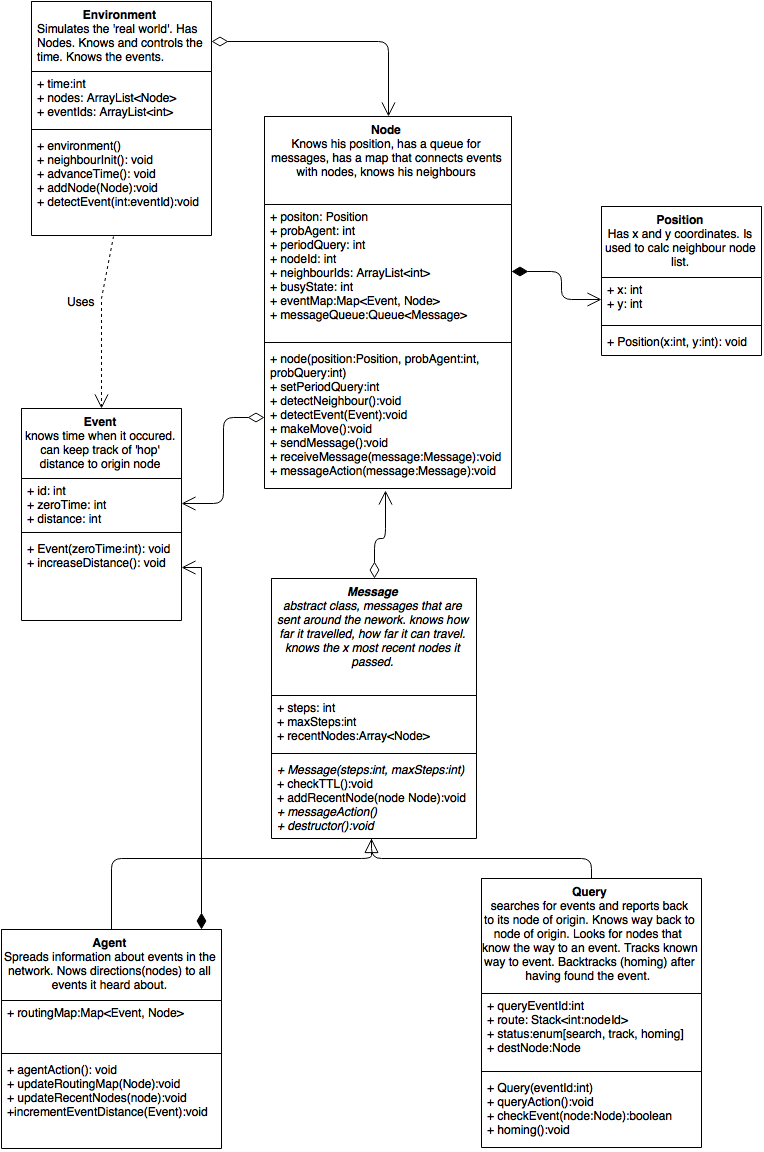
\includegraphics[width=\textwidth]{uml.png}
\caption{\textit{UML diagram for implementing a sensory network application
  that allows testing of the rumour routing algoritm.}}
\label{fig:uml}
\end{figure}



\section{Limitations and Future Development}

\section{Testing Framework}


\section{Individual Contributions}
\subsection{Johan Eklund}
\subsection{Tommie Lindberg}
\subsection{Jakob Lundin}
\subsection{Lorenz Gerber}

\addcontentsline{toc}{section}{\refname}
\bibliography{references}

\end{document}
 
